\documentclass[a4paper]{article}
\special{papersize=200mm,200mm}
\usepackage{geometry}                % See geometry.pdf to learn the layout options. There are lots.
\usepackage{blindtext}
\usepackage[parfill]{parskip}    % Activate to begin paragraphs with an empty line rather than an indent
\usepackage{tikz}
\usetikzlibrary{arrows,automata,shadows,positioning,shapes,fit}
\usepackage{graphicx}
\usepackage{amssymb}
\usepackage{amsmath}
\usepackage{amsthm}
\usepackage{epstopdf}
\usepackage{hyperref}
\usepackage{listings}
\usepackage{subfiles}
\usepackage[utf8]{inputenc}
\usepackage{float}
\usepackage{tikz}
\usepackage{graphicx}
\usepackage{caption}
\usepackage{wrapfig}

\begin{document}

  \begin{figure}
    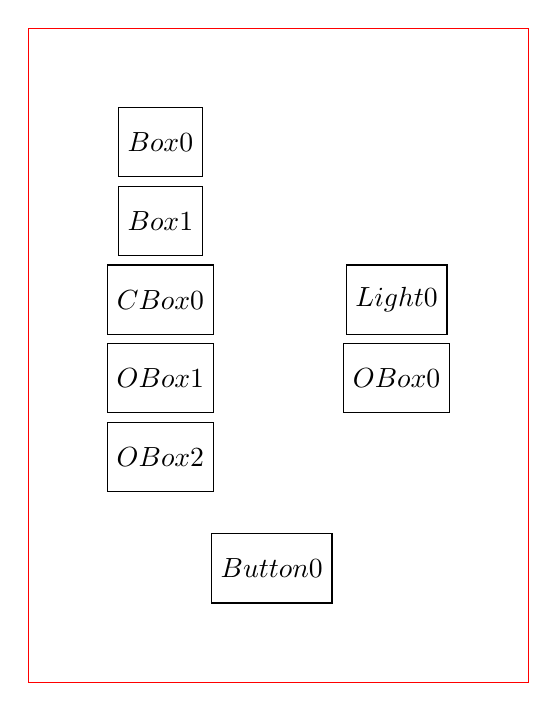
\begin{tikzpicture}
      \node[state,rectangle]  (initIDUser)                            {$Box0$};
      \node[state,rectangle]  (initIDCard)  [below of=initIDUser]     {$Box1$};
      \node[state,rectangle]  (iterBox)     [below of=initIDCard]     {$CBox0$};
      \node[state,rectangle]  (statusLight)
                        [right of=iterBox, node distance = 3cm]       {$Light0$};
      \node[state,rectangle]  (output)      [below of=statusLight]     {$OBox0$};
      \node[state,rectangle]  (checksum1)   [below of=iterBox]        {$OBox1$};
      \node[state,rectangle]  (checksum2)   [below of=checksum1]      {$OBox2$};
      \node[state,rectangle]  (start)       
                      [below right of=checksum2, node distance=2cm]{$Button0$};

      \node (window) [draw=red, fit=(initIDUser) (initIDCard) (iterBox)
                                    (statusLight) (output) (checksum1)
                                    (checksum2) (start), inner sep=1cm] {};
    \end{tikzpicture}
    \label{sketch of the main windows of the GUI.}
  \end{figure}

  \begin{table}
    \begin{tabular}{c | l }
      index number & field description \\ \hline
      $Box0$ & Box for the input of the initial user id \\
      $Box1$ & Box for the input of the initial card id \\
      $CBox0$ & Check box for iterating over several cards \\
      $Light0$ & A status light for the current state including process and writer
      connection \\
      $OBox0$ & Output box for current status notifications \\
      $OBox1$ & Output box for the calculated added checksum \\
      $OBox2$ & Output box for the calculated ibm\_16 checksum \\
      $Button0$ & Button for starting the writing process \\
    \end{tabular}
  \end{table}

\end{document}

